\documentclass{article} % For LaTeX2e
\usepackage{nips13submit_e,times}
\usepackage{hyperref}
\usepackage{url}
\usepackage{graphicx}

\title{Color Detection Under Supervised Learning}


\author{
Cyrus Anderson \\
University of Michigan \\
\texttt{andersct@umich.edu} \\
\And
Jocelyn Bohr \\
University of Michigan \\
\texttt{bjocelyn@umich.edu} \\
\AND
Michael Lu \\
University of Michigan \\
\texttt{lumike@umich.edu} \\
\And
Nghia Vo \\
University of Michigan \\
\texttt{thnghia@umich.edu} \\
}

% The \author macro works with any number of authors. There are two commands
% used to separate the names and addresses of multiple authors: \And and \AND.
%
% Using \And between authors leaves it to \LaTeX{} to determine where to break
% the lines. Using \AND forces a linebreak at that point. So, if \LaTeX{}
% puts 3 of 4 authors names on the first line, and the last on the second
% line, try using \AND instead of \And before the third author name.

\newcommand{\fix}{\marginpar{FIX}}
\newcommand{\new}{\marginpar{NEW}}

\nipsfinalcopy % Uncomment for camera-ready version

\begin{document}

\maketitle

\begin{abstract}

\end{abstract}

\section{Introduction}

\section{Proposed Method}

\subsection{Preprocessing}
// cyrus explain boat stuff \\
Each boat photo we label by hand, marking the color and rectangle around each buoy within about 30 feet from the boat.
From each rectangle, we extract the associated color histogram into a 256x256x256 feature vector, where each entry
represents the frequency of the RGB color associated with the entry index. We then reduce this feature vector to
a vector of size 64x64x64, to make feature vectors less sparse, and to decrease classification time as we are building
this for a real time application.

\begin{figure}[hp]
\begin{center}
%\framebox[4.0in]{$\;$}
\fbox{\rule[0cm]{0cm}{0cm} 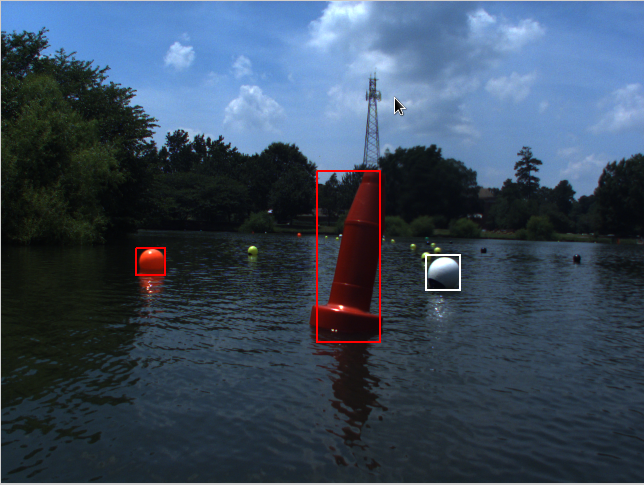
\includegraphics[scale=0.2]{labelling} \rule[0cm]{0cm}{0cm}}
\end{center}
\caption{Labelled photo from boat}
\end{figure}

\subsection{Classification}
In this project, we run our training data with multiclass SVM and multinomial Naive Bayes, and have excellent results. \\\\
We began with SVM beacuse it is a parametric algorithm, thus we do not need to store entire 
training data set to make predictions on the boat. It is also kernelized, which provides us with the flexibility to
create arbitrarily complex boundaries. SVM prediction can be used to calculate confidence values for the
decision by taking the distance from the separating hyperplane, which is a useful measurement. SVM does not make any
assumptions about the underlying distribution of the data. SVM is a very popular algorithm, so it is very good as a baseline
classification algorithm. We used LIBLINEAR for our SVM classification, which utilizes a one-vs-rest multi-class classification
scheme [1]. We achieved very good results with LIBLINEAR, as described later, so we decided not to use any kind of SVM 
kernelization. Using a linear kernel with SVM is preferrable, as it is faster to train and test. Making decisions quickly
is essential to this application, as we want to classify colors at the same rate photos are captured (10 Hz).\\\\
We also used Naive Bayes because it is simple to implement, and performs well even on small sets of training data. Like
SVM, Naive Bayes is parametric, so we do not need to store the entire training data set to make decisions during the
real time application. A parametric classifier is essential, as it is impractical to store all training data on the boat
to make decisions in real time. Naive Bayes is also very fast in training and testing, which is ideal for this application.
The multinomial Naive Bayes classifier works well for classification with discrete features, such as color frequencies of pixels
in a certain section of a photo, or word frequencies of a text document (the classic application). We used MATLAB's multinomial 
Naive Bayes classifier, which performs very well, as described later.

\section{Related Work}
// tommy majority vote and average color algorithm performance \\
// cyrus other related work

\section{Experimental Results}
Using both linear SVM and multinomial Naive Bayes, we achieve excellent accuracy rates, especially compared to
current methods discussed in related works. With enough training examples, both methods achieve over 98\% accuracy. 
Naive Bayes performs marginally better, the advantage of Naive Bayes is emphasized when fewer training examples
are used. Each average accuracy is calculated by selecting a random training set of size $n$, then selecting a
random testing set of size 130 from the remaining data, then train and test classifiers accordingly. The average
accuracy is taken over 10 classification results. Although these results are excellent, we believe one contributing
factor to such great results can be attributed to a fairly homogeneous data set. We do not have enough variation
in our data set, so classification is easier. This problem, and how we intend to solve it, will be discussed
in the future milestones section. Experimental results are shown below.


\begin{table}[hp]
\caption{Linear SVM Average Accuracy}
\begin{center}
\begin{tabular}{ll}
\multicolumn{1}{c}{\bf EXAMPLES}  &\multicolumn{1}{c}{\bf ACCURACY}
\\ \hline \\
50              &89.08 \\
100             &93.77 \\
200             &96.92 \\
400             &97.85 \\
700             &98.38 \\
\end{tabular}
\end{center}
\end{table}

\begin{table}[hp]
\caption{Multinomial Naive Bayes Average Accuracy}
\begin{center}
\begin{tabular}{ll}
\multicolumn{1}{c}{\bf EXAMPLES}  &\multicolumn{1}{c}{\bf ACCURACY}
\\ \hline \\
50              &92.85 \\
100             &96.54 \\
200             &97.31 \\
400             &98.38 \\
700             &98.31 \\
\end{tabular}
\end{center}
\end{table}

\section{Future Milestones}
One problem with our method we have identified is that the data set we are using is from one log, resulting in a very
homogenous data set. Within one week from the due date of the progress report, we plan to label at least another 1000-5000 
buoys, including many more blue and green buoys, and more buoys in varied lighting conditions. We hope that after running
our algorithms on this data set with variation, we have a more realistic classification accuracy, which will perform better
during the real application. We also want to try to add a feature which encodes the direction of lighting, to be completed
within two weeks. One idea we have as an extension to this color classification project is implementing a segmentation 
algorithm to identify buoy boundaries under unsupervised learning, then do color classification with or current supervised 
learning algorithms. We are considering an extension to this project as we have achieved excellent results so far, thus
we don't have much room for further improvement for the rest of the semester. We will discuss what we should pursue as
a possible extension with the EECS445 staff. 
 

\section{Conclusion}

// michael do conclusion

\subsubsection*{References}

// michael do references

References follow the acknowledgments. Use unnumbered third level heading for
the references. Any choice of citation style is acceptable as long as you are
consistent. It is permissible to reduce the font size to `small' (9-point) 
when listing the references. {\bf Remember that this year you can use
a ninth page as long as it contains \emph{only} cited references.}

\small{
[1] Alexander, J.A. \& Mozer, M.C. (1995) Template-based algorithms
for connectionist rule extraction. In G. Tesauro, D. S. Touretzky
and T.K. Leen (eds.), {\it Advances in Neural Information Processing
Systems 7}, pp. 609-616. Cambridge, MA: MIT Press.

[2] Bower, J.M. \& Beeman, D. (1995) {\it The Book of GENESIS: Exploring
Realistic Neural Models with the GEneral NEural SImulation System.}
New York: TELOS/Springer-Verlag.

[3] Hasselmo, M.E., Schnell, E. \& Barkai, E. (1995) Dynamics of learning
and recall at excitatory recurrent synapses and cholinergic modulation
in rat hippocampal region CA3. {\it Journal of Neuroscience}
{\bf 15}(7):5249-5262.
}

\end{document}
